\documentclass[tikz,border=8pt]{standalone}
\usetikzlibrary{arrows.meta,calc}
\begin{document}
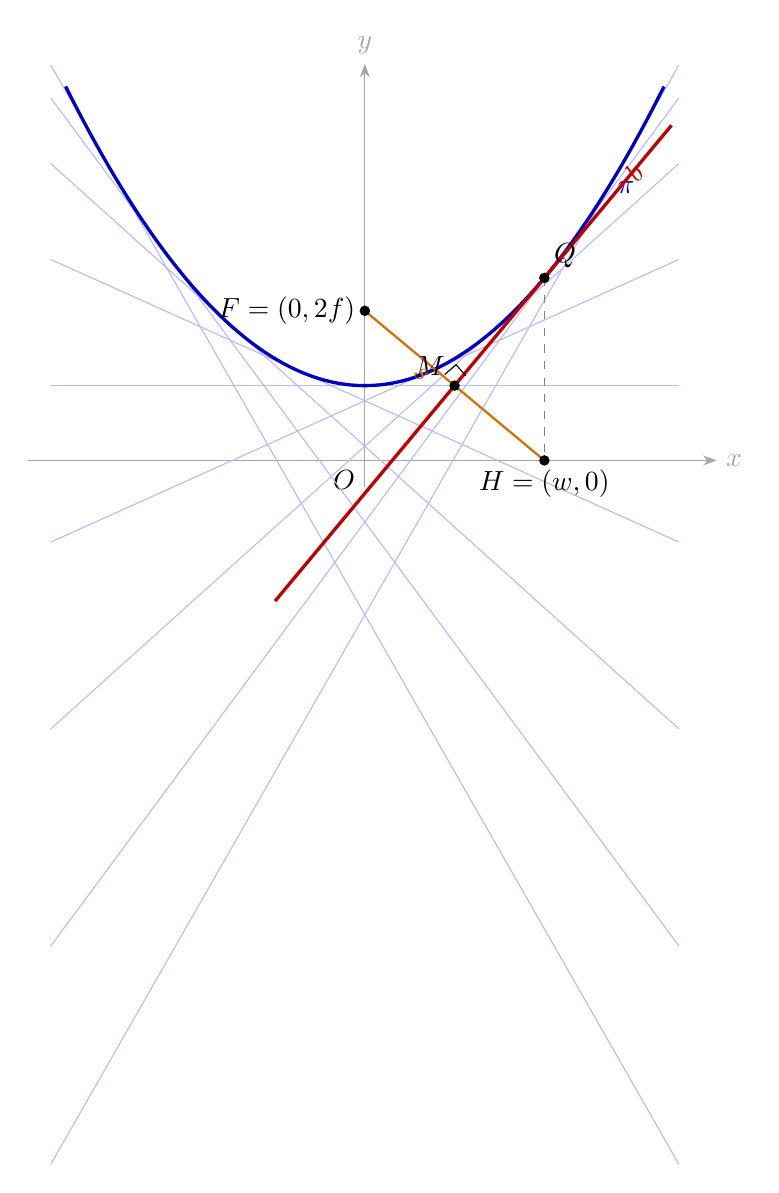
\begin{tikzpicture}[>=Stealth,scale=0.95]
  % Use f=1: directrix y=0, focus (0,2), parabola y=1+x^2/4.
  \draw[->,gray!70] (-4.5,0) -- (4.7,0) node[right] {$x$};
  \draw[->,gray!70] (0,-0.35) -- (0,5.3) node[above] {$y$};
  \node[below left] at (0,0) {$O$};

  \foreach \w in {-3.5,-2.7,-1.8,-0.9,0,0.9,1.8,2.7,3.5} {
    \draw[blue!28,thin,domain=-4.2:4.2]
      plot (\x,{1 + (\w*\x)/2 - (\w*\w)/4});
  }
  \draw[blue!75!black,very thick,domain=-4:4,samples=100]
    plot (\x,{1 + (\x*\x)/4});
  \node[blue!75!black,right] at (3.25,3.65) {$\pi$};

  \coordinate (F) at (0,2);
  \coordinate (H) at (2.4,0);
  \coordinate (M) at (1.2,1);
  \coordinate (Q) at (2.4,2.44);
  \draw[orange!85!black,thick] (F) -- (H);
  \draw[red!75!black,very thick,domain=-1.2:4.1]
    plot (\x,{1 + (2.4*\x)/2 - (2.4*2.4)/4});
  \draw[dashed,gray] (Q) -- (H);

  \fill (F) circle (2pt) node[left] {$F=(0,2f)$};
  \fill (H) circle (2pt) node[below] {$H=(w,0)$};
  \fill (M) circle (2pt) node[above left] {$M$};
  \fill (Q) circle (2pt) node[above right] {$Q$};
  \node[orange!85!black,rotate=-40] at (0.75,1.15) {$s$};
  \node[red!75!black,rotate=50] at (3.6,3.85) {$b$};
  \draw ($(M)+(-0.13,0.15)$) -- ($(M)+(0.02,0.28)$) -- ($(M)+(0.15,0.13)$);
\end{tikzpicture}
\end{document}
